\chapter{Existing technologies}

In the beginning, we will observe conventions in web applications, and we will map ways of user interaction with the applications to utilize it later in the proposed solution.
We will explore a server-side web application using PHP language and a client-side web application using Javascript language in other to obtain these observations.
Afterward, it will present a WebAssembly, which will be followed by the existing project relating to run PHP in a browser.
It will give short information about the .NET platform and C\# language.
In the end, it will introduce Blazor and Peachpie, which will be integrated.

\section{PHP and server-based web application}

The basic principle of obtaining a web page is a request-response protocol, where a client sends a request for the web page using an HTTP protocol and receives a response with requested data.
An HTTP protocol uses a dedicated format of messages for communication.
The protocol does not require any authentication at all.
Statelessness is a typical characteristic of the protocol.
A server has to retain information about clients and add additional information to the messages in order to distinguish between the clients.
\par
Since the server contains all business logic, a browser has to send necessary data for required actions by an HTTP message.
The data are usually encoded as a part of an URL address or in the HTTP message body.
HTML presents a tag Form that makes sending the data easier for a client.
Listing \ref{lst:PHP} contains an example of a Form tag.
The form can contain other tags, which are displayed as various types of fields.
A client fills these fields, and the browser sends the data as a new HTTP request to the server.
We can specify how the data will be encoded.
Get method is one of the basic ways.
It encodes the data as a pair of keys and its values to the query part of the URL.
There is a example of an URL
\url{http://www.example.com/index.php?par1=hello\&par2=2\&arr=hello\&arr=2}.
A query part begins with a question mark.
Parameters of the query part are described in the table \ref{tab01:query}.
\begin{table}[h]
\centering
\begin{tabular}{l@{\hspace{1.5cm}}D{.}{,}{3.2}D{.}{,}{1.2}D{.}{,}{2.3}}
\pulrad{\textbf{Key}} & \pulrad{\textbf{Value}}\\
par1 & hello\\
par2 & 2\\
arr  & [hello, 2]\\
\end{tabular}
\caption{Parameters of the query part.}
\label{tab01:query}
\end{table}
Another method is called post, which encodes it in the request body, which does not appear in the URL.
\par
PHP \squarecite{5} was designed for user page templating on the server-side.
It has been adjusted gradually to enable writing application logic.
PHP is an interpreted language maintained by The PHP Group.
We will describe the language by using listing \ref{lst:PHP} as an example.
\par
\begin{minipage}[c]{0.95\textwidth}
\begin{lstlisting}[basicstyle=\small, caption=A PHP code.,
  language=PHP, label={lst:PHP}]
<?php
    inlude("header.php");
?>

<h1>Superglobal POST</h1>
<?php
	foreach($_POST as $key => $value) { ?>
	<p><?php echo $key; ?> => <?php echo $value; ?></p>
<?php } ?>

<h1>File content:</h1>
<p>
<?php 
	if($_FILES["file"])
	{
		echo file_get_contents($_FILES["file"]["tmp_name"]);
	}	
?>
</p>

<form action="/index.php" method="post">
  <label for="name">Name:</label>
  <input type="text" id="name" name="name"><br>
  <label for="file">File:</label>
  <input type="file" id="file" name="file"><br>
  <input type="submit" value="Submit">
</form>

<?php
    inlude("footer.php");
?>
\end{lstlisting}
\end{minipage}
\par
An HTML interleaving has appeared to be a helpful method for data binding.
The feature allows inserting a PHP code between HTML.
These fragments do not have to form individual independent blocks of code closed in curly brackets.
The interleaving is related to code execution when an interpreter executes a script from top to bottom. Everything outside a PHP section is copied into the body of the request.
\par
We do not see any specification of type next to variables.
This is because the type system is dynamic.
A variable represents just a reference to the heap.
Its type is determined during runtime. 
\par
PHP has superglobals \squarecite{6}, which are built-in variables accessible from all scopes of the script.
Following superglobals are relevant to the thesis.
The \$\_GET variable stores parsed query part of the URL.
The \$\_POST variable stores variables which are sent by post method.
The \$\_FILES variable contains uploaded files.
\par
\change[inline]{Maybe add information about SESSION.}
We can divide code in several ways.
Global functions are the most notable characteristic of PHP despite wide-spread object-oriented programming.
They are defined in the global scope and accessible from anywhere.
The next option is an object inspired by object-oriented programming.
There is also namespace support.
We can include a PHP code from other scripts. 
The execution continues after the inclusion, which is a common execution of the defined script.
\par
The nature of the request-response semantic usually results in a one-way pass of the application.
After dealing with a request, the whole application state is terminated.
One of the well-known design patterns relating to PHP is the Front controller.
Usually, the main script invokes other parts of the program, based on the request, to deal with it and send the response back.
The idea of this pattern can be shown in listing \ref{lst:PHP}.
In the beginning, we delegate header rendering to header.php script.
Then we render the body and include footer.php, which cares about the proper ending of the HTML page.
\par
Uploaded files sent by the client reside in two places.
The file's information is stored in \$\_FILES.
The uploaded file is saved as a temporary file, and standard reading operations can obtain the content.
This is demonstrated in the previously mentioned example.

\section{Javascript and client-based web application}

Since a client-based web application aims to do a major business logic in a browser, it needs to control the rendered page and access a web interface providing additional services.
The interface is usually available from Javascript.
We will start with a description of loading Javascript in a browser.
We will introduce a page representation in a browser alongside page events.
In the end, we will present Javascript as a scripting language for the creation of a responsive web page.
\par
The process of generating a web page follows several steps.
A browser parses the HTML line by line. If a script occurs, the browser starts to execute the code.
The order of processing is important for manipulation with an HTML structure.
This limitation can be solved by web events mentioned later, but
it is a convention to add scripts to the end of the body part after all HTML tags are parsed.
\par
We can image a web page as an XML tree.
Its nodes are tags or text fragments, and its edges connect nodes with their children.
One representation of this tree is Document Object Model (abbreviated DOM).
Each node is represented by an object with special parameters relating to HTML and CSS. 
The nodes can contain other nodes representing their children.
Afterward, there is a document node representing the whole document together with its root node.
\par
Events are the most common method of how to react to changing a web page state.
Every event can have some handlers(listeners).
Whenever an event occurs, it calls all its listeners.
There are many event types, but we will mention the ones that are important for us.
HTML tags are the most common entities, which can have some events.
For example, a button has an event onclick which triggers when a client clicks on the button as we ca see in listing \ref{lst:Javascript}. 
Other events can represent a state of a page like onload which fires when the whole HTML document is parsed.
\par
A browser provides more APIs valuable for the application, like fetching extra data from a server or local storage.
These APIs are mentioned as Web API \squarecite{7}.
\par
ECMAScript is a Javascript standard recommending across browsers.
It is abravieted as ES.
We can see later an abbreviation ES2015 which relates to the ECMAscript version.
Javascript is a high-level language usually executed by a browser's dedicated Javascript engine but can also be run on a desktop.
Node.js is an example of a Javascript runtime running outside a browser.
Listing \ref{lst:Javascript} will be used to show the language in the simple scenario.
The page contains a button that invokes an alert with a second delay when a client clicks on it.
\par
\begin{minipage}[c]{0.95\textwidth}
\begin{lstlisting}[basicstyle=\small, caption=A Javascript code., label={lst:Javascript}]
<!DOCTYPE html>
<html>
	<head>
	</head>
	<body>
		<button id="alert">Click to alert</button>
		<script>
			var handler = function (arg) {
				var timer = new Promise((resolve) => {
					setTimeout(resolve, 1000);
				}); 
        
				timer.then(() => window.alert("Hello world."));
			};  

			var button = window.document.getElementById("alert");
			button.addEventListener("click", handler);
		</script>
	</body>
</html>
\end{lstlisting}
\end{minipage}
\par
At first glance, we can see the type system is dynamic as well as PHP.
A window is an essential global variable, which is an object representing the browser window of the running script.
The window object consists of all defined global variables.
It also contains a document property, which is an API for manipulating the DOM tree.
We can see the usage of the document property in the example.
Javascript object is often used as a wrapper of Web APIs.
\par
Functions are first-class citizens in Javascript.
We can treat them as common variables.
Javascript supports an event-driven style that helps to react to events conveniently.
There is a handler assigned to the click event in the listing.
\par
\change[inline]{Maybe add a section about async functions. Compare it with PHP}
Javascript is single-threaded, which can be confusing with its constructs for promises.
The promise is a structure representing an unfinished process.
These processes can be chained.
However, the structure can give an illusion of multi-threading. It uses the scheduler for planning the next task executed by the main thread.
The single thread is critical for blocking operations which causes thread freezing.
\par
Web workers \squarecite{11} are a browser feature enabling to run the script in the background.
There are wrapped as Worker objects.
The worker limitation is communication with UI thread only by handling message events. 
Messages have to be serialized and deserialized.
\par
Javascript module is the last thing, which we will need to present.
It gathers a collection of code.
Global entities of this code can be exported to another script.
These exports make an API of the module.
The module's advantage is defining the API and hiding the internal code, which is not relevant for the user.

\section{WebAssembly}

WebAssembly \squarecite{9} is a new code format that can be run in today's browsers. 
It has a compact byte format, and its performance is near to a native code. 
WebAssembly is designed to be a compiling target of popular low-level languages like C or C++ due to its memory model.
It results in the possibility to run other languages in a browser because its runtime is often written in C or C++. 
The advantage of this format is a similarity with Javascript modules ES2015 after compilation into a machine code. 
This enables browsers to execute it by a JavaScript runtime. 
So its security is as good as a code written in Javascript. 
Because of the same runtime, WebAssembly can call Javascript and vice versa.
\par
Threads \squarecite{10} support is currently discussed nowadays and appears to be promising.
After all, new versions of Google Chrome experiments with proper multi-threading support despite the chance of vulnerability.
A replacement of multi-threading can be Web workers mentioned in Javascript section.
\par
Despite supporting to run WebAssembly in a browser, the browser cannot load it as a standard ES2015 module yet.
WebAssembly JavaScript API was created in order to be able to load a WebAssembly to a browser using JavaScript.

\section{Project PHP in browser}

The project \squarecite{2} aims to use compiled PHP interpreter into WebAssembly, which allows evaluating a PHP code.
The page has to import a specialized module php-wasm. 
A PHP code is evaluated by writing a specialized script block or manually by JavaScript and API.
PHP can afterward interact with JavaScript using a specialized API.
At first glance, that might be a good enough solution, but they are several parts that can be problematic due to PHP semantics.
The solution doesn't solve superglobals. 
This is reasonable because this is the server's job, but you are not able to get information about a query part or handling forms without writing a JavaScript code.
The next problem is navigating how a script can navigate to another script without an additional support code which has to be JavaScript.

\section{C\# and .NET 5}

We have to introduce the Common Language Infrastructure (abbreviated CLI) \squarecite{18} before diving into .NET.
CLI is a specification describing executable code and runtime for running it on different architectures.
CLI contains descriptions of a type system, rules, and the virtual machine (runtime), which executes specified Common Intermediate Language (abbreviated CIL) by translating it to a machine code. 
The virtual machine is often named CLR (Common Language Runtime).
CIL's advantage is a compilation target of languages like C\#, F\#, and C++\\CLI, which gives us great interoperability.
.NET Framework, .NET 5, and Mono are implementations of CLI.
\par
.NET 5 \squarecite{17} is the last version of .NET Core, which is a cross-platform successor to .NET Framework.
From now on, we will refer .NET 5 as .NET, since it should be the only supported framework in the future.
.NET is a free and open-source project primarily developed by Microsoft.
It consists of many libraries, runtime for executing CIL.
The libraries can represent whole frameworks like ASP.NET, which aims to web development.
A large collection of code is usually compiled into an assembly containing the code and additional metadata.
As assembly can represent either library or an executable program.
\par
Mono aims to mobile platforms. 
Recently, they started to support compilation \squarecite{12} into WebAssembly.
This support allows executing CIL inside browsers.
The compilation has two modes.
The first one is compilation Mono runtime with all using assemblies.
The second only compile Mono runtime, which then can execute .dll files without further compilation of them into WebAssembly.
A consequence of these compilations into WebAssembly is enabling to call Javascript and WebAPI from C\#.
\par
C\# is a high-level language using strong typing and a garbage collector.
It has a multi-paradigm, but its common characteristic is the objected-oriented style.
These features cause that C\# is a good language for a huge project which needs discipline from developers to hold the code understandable and manageable.
C\# is used on the server-side as well as PHP.

\section{Blazor}

Blazor is a part of the open-source ASP.NET framework.
Blazor allows creating client-side web applications written in C\# language.
Blazor framework offers two hosting models \squarecite{13} which have different approaches to creating web applications. 
The first one is referred to as Blazor Server App and represents a server-side web application using specific communication between a client for better functionality.
An interesting innovation is SignalR which is a communication protocol between the server and a client.
The thesis uses the second model, which Microsoft refers to as Blazor WebAssembly App, enabling moving business logic to a client-side without using Javascript.
\par
From now on, I will use Blazor App to refer Blazor WebAssembly App.
The application can be hosted by a standalone project representing a standard ASP.NET web server.
It will become useful for further server settings, and the proposed solution utilizes it.
The division enables a choice of a place for the implementation of business logic.
If there is a bad connection, we can move the majority of business logic to the client and use the server for connection to a database; otherwise, we can use the client only for rendering the page. It consists of the following components. 
When we choose the template, there are two main projects to describe.
\par
The first one is a server, which serves the Blazor App to a client.
There is nothing special about the project expects a middleware, which provides the Blazor files.
A middleware is a segment of an HTTP request pipeline, which cares about some functionality related to processing the request.
\par
We will describe the second project (Blazor App) in figure \ref{img01:project} to explain basic entities and their interaction with each other.
\par
\begin{figure}[H]\centering
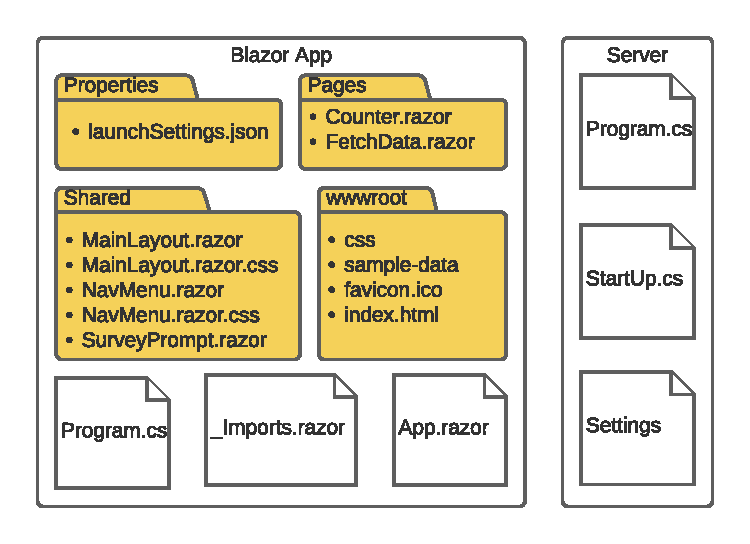
\includegraphics{./img/ProjectStructure}
\caption{A basic Web Assemby App project.}
\label{img01:project}
\end{figure} 
\par
We will start with a new format Razor to get familiar with it.
Razor is a markup language interleaving HTML with C\#.
Razor uses special sign at with keywords to identify C\# code in HTML.
Razor's compilation results in a pure C\# code representing the web page fragment.
We can see an example of Razor in listing \ref{lst:razorpage}.
\par
Although the format is self-explaining, we point to the keywords.
The first line begins with a page keyword determining a part of the page's URL.
The next keyword is inject, representing a HttpClient service injection. 
An if keyword determines a standard condition.
A code keyword contains a regular C\# code, which can be used in the whole razor file.
\par
A Razor file is transformed into a C\# dedicated class.
The class inherits from ComponentBase or implements IComponent, which provides necessary methods for rendering the page.
Components can be arbitrarily put together in order to form the desired page.
We can see the generated Component from listing \ref{lst:razorpage} in listing \ref{lst:component}.
\par
We can assign the Razor keywords to parts of the code in the listing.
Page keyword stands for Route attribute.
Inject keyword stands for parameter attribute. The parameter is assigned by a dispatcher, mentioned later, during the initialization.
Code keyword is a part of class content.
Another markup is transformed into calling a specialized method in the BuildRenderTree function, which describes the page content for rendering. 
There will be more information about rendering later in this section.
\par
\begin{figure}
\begin{minipage}[c]{0.95\textwidth}
\begin{lstlisting}[basicstyle=\small, caption=Example of Razor page., label={lst:razorpage}]
@page "/example"
@inject HttpClient Http

<h1>Example</h1>
@if (!loaded)
{
    <p>Loading...</p>
}
else
{
    <p>Ticks: @ticks</p>
}

@code {
    private bool loaded = false;
    private int ticks = 0;

    protected override async Task OnInitializedAsync() {
        ticks = await Http.GetFromJsonAsync<int>("ticks.json");
        loaded = true;
    }
}
\end{lstlisting}
\end{minipage}
\begin{minipage}[c]{0.95\textwidth}
\begin{lstlisting}[basicstyle=\small, caption=Razor page generated to the C\# class., label={lst:component}]
[Route("/example")]
public class Index : ComponentBase {
	private bool loaded = false;
	private int ticks = 0;
	
	[Inject] private HttpClient Http { get; set; }

	protected override void BuildRenderTree(RenderTreeBuilder __builder) {
		__builder.AddMarkupContent(0, "<h1>Example</h1>");
		if (!loaded)
		{
			__builder.AddMarkupContent(1, "<p>Loading...</p>");
			return;
		}
		__builder.OpenElement(2, "p");
		__builder.AddContent(3, "Ticks: ");
		__builder.AddContent(4, ticks);
		__builder.CloseElement();
	}

	protected override async Task OnInitializedAsync() {
		ticks = await Http.GetFromJsonAsync<int>("ticks.json");
		loaded = true;
	}
}
\end{lstlisting}
\end{minipage}
\end{figure}
\par
\change[inline]{Add asynchronous functinons and component's lifecycle.}
\par
We return to the project description. 
Folders Pages and Shared contains parts of Blazor pages written in Razor.
\_Imposts.razor contains namespaces, which are automatically included in others .razor files.
The next folder is wwwroot, containing static data of the application.
We can see index.html, which cares about loading parts of the Blazor application to the browser.
\par
We will describe the loading of Blazor into the browser to fully understand the interaction between Blazor and the browser.
We have the server, the Blazor App, and other optional user's defined projects. 
When we start the server and tries to navigate the web application, the following process is done.
The server maps the navigation to index.html and sends it back.
\par
\begin{minipage}[c]{0.95\textwidth}
\begin{lstlisting}[basicstyle=\small, caption=A Javascript code., label={lst:Javascript}]
<body>
    <div id="app">Loading...</div>
    <div id="blazor-error-ui">
        An unhandled error has occurred.
		...
    </div>
    <script src="_framework/blazor.webassembly.js"></script>
</body>

\end{lstlisting}
\end{minipage}
\par 
The index.html contains a script initializing Blazor.
The first step is to load all resources, which are defined in a separate file.
Blazor cuts all unnecessary .dll to reduce the size.
For this reason, all .dll has to be used in the Blazor App code in order to be contained in the file. 
These resources contain Mono runtime compiled into WASM, additional supporting scripts, and all .dll files containing the whole application (Blazor App with referenced libraries).
The supporting scripts initiate the runtime a run it.
The runtime includes the .dll into the application and calls the Main method in Program.cs defined in Blazor App project.
We can see the process in figure \ref{img02:wasm}.
\par
\begin{figure}[H]\centering
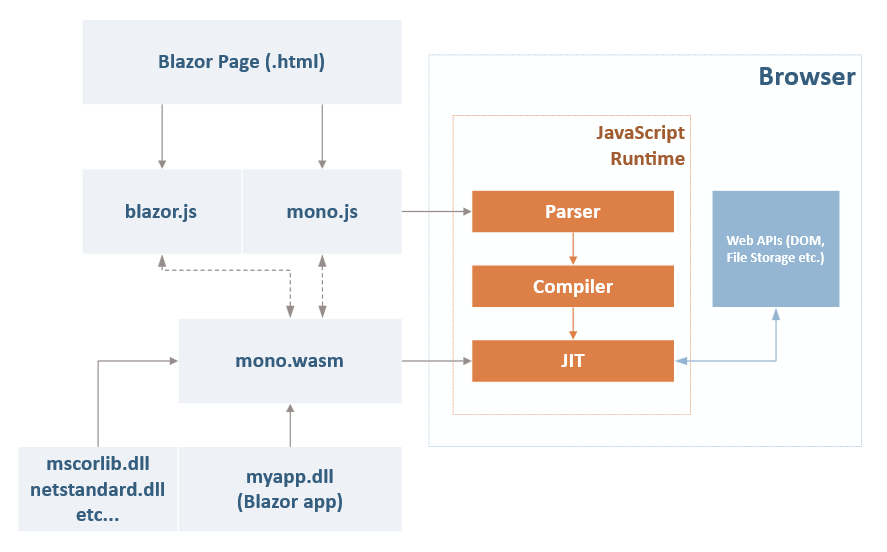
\includegraphics[width=140mm, height=100mm]{./img/BlazorExecution}
\caption{Running a Blazor WebAssembly App on client-side.}
\label{img02:wasm}
\end{figure}
\par
Main method uses WebAssemblyHostBuilder to set the application.
It defines services, which will be able through the dispatcher.
It set a root component, which will be rendered as the first.
The host is run.
Afterward, the application provides the dispatcher, cares about rendering, and communicates with the runtime to offer interop with Javascript.
\par
App.razor is the last file for clarification.
It is the root component in default.
It contains a specialized component, a Router, enabling to navigate the pages.
\par
In the end, we will describe page navigation and rendering and handling events.
The navigation \squarecite{14} can be triggered by an anchor, form, or filling up the URL bar.
The URL bar is handled separated by a browser.
JavaScript can influence the remainings elements.
Blazor App handles only an anchor.
After clicking on an anchor, a navigation event is fired.
One of the handlers is a javascript function, which invokes C\# method through Mono WASM. 
The method represents a navigation handler in Blazor App.
A user can add listeners to the handler, but the Router implements default behavior for navigating.
The Router finds out all components, which implements an IComponent interface, by a reflection, and tries to render the page according to path matching RouteAttribute of a component whenever the navigation is triggered.
The navigation can be redirected to the server if there is no match.
\par
The rendering process begins with the Renderer initialized in the application's builder.
Render cares about representing a virtual DOM of the page, creating a page's updates, and updating it with the runtime interop's support.
Renderer provides RenderTreeBuider for describing page contents.
The builder provides an API for adding various types of content to Batch, which is a specialized structure for describing previous and present virtual DOM changes.
The changes are recognized by a diff algorithm, which is used to reduce changing a DOM directly in a browser to its demanding performance.
The usage of RenderTreeBuilder is complicated due to the algorithm.
The purpose of Razor is to make an implementation C\# method BuildRenderTree easier.
When the Renderer prepares the Batch, it calls specialized Javascript API for changing the page through Mono runtime.
\par
The diff algorithm is used to minimize the browser's DOM  update after all components used RenderTreeBuilder to render their content.
This algorithm used sequence numbers for parts of HTML to identify modified sections.
Sequence numbers respond to an order of RenderTreeBuilder's instructions in the source code.
A benefit of this information is detecting loops and conditional statements to generating smaller updates of DOM.  
\par
Event handling is just clever usage of the Renderer with dedicated Javascript API for updating, where the API registers the listener.
When the event is fired, the listener invokes C\# method representing the handler through the WASM runtime.
\par
Blazor provides API for invoking Javascript functions and vice-versa.
\par

\section{Peachpie}

Peachpie \squarecite{16} is a modern compiler based on Roslyn and Phalanger project.
It allows compiling PHP into a .NET assembly, which can be executed alongside standard .NET libraries.
Peachpie introduces several structures representing states, scripts, and variables of PHP written in Csharp.
The first of them is a context representing one request to PHP code.
The context consists of superglobals, global variables, declared functions, declared and included scripts.
The possibility of saving the context and using it later is a significant advantage used in the solution.
The context can also be considered as a configuration of the incoming script's execution.
All information about a request can be arranged to mock every situation on the server-side.
The compiler offers a dedicated type of assembly for PHP libraries.
Using this assembly can add additional functions, which can provide an extra nonstandard functionality as an interaction with a browser.
Another advantage of the compiler is the great interoperability between PHP and .NET.
An option to work with Csharp objects, attributes and calling methods will become crucial for achieving advanced interaction between Blazor and PHP.

\change[inline]{Saving script information in the assembly}
\change[inline]{Inheriting the CSharp classes}

However, there are limitations following from differences in the languages and the stage of development.
Availability of PHP extensions depends on binding these functions to CSharp code which gives equivalent results. The time and memory complexity of this code can be tricky in Blazor.
The previously mentioned interoperability has limits as well.
Csharp constructs like structs and asynchronous methods are undefined in PHP.


